\documentclass[10pt]{beamer}
\usepackage{braket}
\usepackage{graphicx}
\usepackage{latexsym}
\usepackage{amssymb,amsmath}
\usepackage{color}

\usepackage{caption}
\usepackage{subcaption}

\usetheme{Warsaw}
\title[MC Simulation of the Ising Model]
{Monte Carlo Simulation \\ 
of the Ising Model}
\author{
Onur Kaplan}
\institute[I.T.U.]{
%\includegraphics[scale=0.3]{../figures/sunum/intro2} \\
Advanced Physics Project Laboratory \\ 
Project Presentation \\
Istanbul Technical University}
\date{7 Jan 2014}

\begin{document}

\begin{frame}
\titlepage
\end{frame}
\note{
Hello everyone, my name is Onur Kaplan.
Welcome to my senior project presentation 
on the application of the density matrix 
renormalization group method to one-dimensional 
single particle quantum mechanics problem.
}

\begin{frame}{\title=Table of contents}
\tableofcontents[section,subsection]
\end{frame}
\note{
Let me start by giving an outline of my talk. 

In the first part I will talk about the DMRG 
in general which in usual consists of 
two algorithms: the infinite size algorithm 
and the finite size algorithm.

In the second part, I will talk about the 
application of this method to the single particle 
case\dots

}

\section{Monte Carlo Method}
\begin{frame}
\frametitle{Monte Carlo Method}
\begin{itemize}
\item Statistical approach for physical processes. \\
\item Statistical approach to compute integrals with samples. \\
\item Statistical approach to analyze properties of large systems with using limited states of the system \\
\end{itemize}
\end{frame}
 \note{

Monte Carlo method is a statistical approach to simulate physical processes and it is used to compute integrals using random states, called samples. By  using these samples we approximate the integrals in discrete manner.

Also, with Monte Carlo method, we can estimate properties of large systems with using several states of the system as in Ising Model.

}

\subsection{Estimation of Expected Value}
\begin{frame}
\frametitle{Estimation of Expected Value}
For Maxwell-Boltzmann dist. expected value of Q;
\begin{equation}
\langle Q \rangle = \frac{\sum\limits_{\mu} Q_\mu e^{-\beta E_\mu}}{\sum\limits_{\mu} e^{-\beta E_\mu}} \qquad \beta = 1/kT
\end{equation}
With respect to Monte Carlo method, expected value of Q;
\begin{equation}
Q_M = \frac{\sum\limits_{i=1}^M {Q_\mu}_i {{P_\mu}_i}^{-1} e^{-\beta {E_\mu}_i}}{\sum\limits_{j=1}^M {{P_\mu}_j}^{-1} e^{-\beta{E_\mu}_j}}
\end{equation}
\begin{equation}
P_\mu = Z^{-1} e^{-\beta E \mu} 
\end{equation}
Then, estimator of expected value is;
\begin{equation}
Q_M = \frac{1}{M} \sum\limits_{i=1}^M {Q_\mu}_i 
\end{equation}


\end{frame}
\note{

Let's assume that we have a property of a system which is distributed with 
respect to maxwell boltzmann distribution. Expectation value of this 
quantity is given in 1. To calculate it we have to consider all values of the 
property in the system. But, we can estimate this value with using Monte 
carlo method. With choosing these property values in a probability 
distribution, p mu, we can estimate it. In this case this estimate is in the 
form of (2). Also, it is obvious that if we choose these property values with 
respect to maxwell-boltzmann distribution, we will get better 
approximation. because, properties also distributed wrt maxwell 
boatsmann distribution. Hence, p mu is in the form of (3). If we use (3) in 
(2), then our estimation of expected value is (4). 

Z is a normalization constant for probability Pμ. 

}
  
\subsection{Getting Samples with Desired Probability Distribution}
\begin{frame}
\frametitle{Getting Samples with Desired Probability Distribution}

Aim: Sample states so that each one appear with its correct probability distribution (In the form of Maxwell-Boltzmann distribution for Ising Model as in eqn. (3)) \\

\begin{itemize}
\item \small Markov Process: \\
\begin{equation}
\sum\limits_{\nu} P(\mu \rightarrow \nu) =1
\end{equation}
\item \small Markov Chain: \\
Repeated Markov Processes. \\
A long run of Markov Chain = Correct Distribution \\
\end{itemize}

\end{frame}
  \note{
  
Now, we want that we choose these samples with respect to Maxwell-
boltzmann distribution. We sample these states of the system in a chain 
with using Markov-Chain sampling method. Firstly, let's define a ring of 
this chain. It is Markov Process. If we are in a state mu then probability to 
move another state nu is given by Transition probability P mu nu with 
respect to Markov Process. Also, it is obvious that if we are in a state, sum 
of probability of move to another state and not move any state is 1 as in 
(5). If we use markov processes repeatedly, we get markov chain. After a 
long run of Markov chain we can achieve states which obey maxwell-
boltzmann distribution. 

Firstl of all, to get a stable probability distribution for states at the end of 
the markov chain, we should satisfy equilibrium condition.
  
}

\begin{frame}
\begin{itemize}
\item \small Equilibrium condition: \\
\begin{gather}
\sum\limits_{\nu} P_\mu P(\mu \rightarrow \nu) = \sum\limits_{\nu} P_\nu P(\nu \rightarrow \mu)  \\
P_\mu  = \sum\limits_{\nu} P_\nu P(\nu \rightarrow \mu)
\end{gather}
\item \small Detailed balance: \\
\begin{gather}
 P_\mu P(\mu \rightarrow \nu) = P_\nu P(\nu \rightarrow \mu) \\
\frac{P(\mu \rightarrow \nu)}{P(\nu \rightarrow \mu)} = \frac{P_\nu }{P_\mu } = e^ {-\beta (E_\nu - E_\mu)}
\end{gather}
%\item \small Dynamic Equilibrium: \\ 
%If we reach dynamic equilibrium, probability distribution rotates around different values. This rotation is called limit cycle.
%\item \small Simple Equilibrium: \\
%No limit cycle. 
\end{itemize}
Want to satisfy equations (5) and (9). \\
\end{frame}
  \note{
  
Equilibrium condition states that, transitions into a state and out of that state must be equal. After this condition is achieved, our probability distribution of states at the end of the Markov chain will be a stable distribution because after equilibrium, probability distribution will not change on average. 

Also, to achieve desired probability distribution, which is in the form of Maxwell-Boltzmann distribution, after achieving the equilibrium, we have to satisfy detailed balance condition.

If we look at detailed balance condition, it also includes equilibrium condition which is described above. Hence, if detailed balance is satisfied, then equilibrium condition will also be satisfied.

Hence, if we satisfy equation (5) and (8), we will create states with probabilities P mu. We want to satisfy Maxwell-Boltzmann distribution, therefore we should choose pμ in the form of Maxwell-Boltzmann probabilities. It's done by using detailed balance condition (9).

Hence if we satisfy (5) and (9), we will get a succession of states which obey Maxwell-Boltzmann distribution. 

%Also, To achieve intended probability distribution, we should reach simple equilibrium, by avoiding dynamic equilibrium. Because, if dynamic equilibrium is achieved, our probability values cycles between a number of probability distribution 
  
%If dynamic equilibrium is achieved, our probability values cycles between a number of probability distribution. Hence, we will not reach desired probability distribution because it only cycles. Hence, we want to get rid of dynamic equilibrium. 

%To get rid of dynamic equilibrium, we should satisfy Detailed balance condition.

-> Dynamic equilibrium ve stable equilibrium cıkarıldı.

} 

\begin{frame}
\centering
Acceptance ratio and Selection Probabilities: 
\begin{equation}
P(\mu \rightarrow \nu) = g(\mu \rightarrow \nu) A(\mu \rightarrow \nu)
\end{equation}
\begin{equation}
\frac{P(\mu \rightarrow \nu)}{P(\nu \rightarrow \mu)} = \frac{g(\mu \rightarrow \nu)A(\mu \rightarrow \nu)}{g(\nu \rightarrow \mu)A(\nu \rightarrow \mu)} = \frac{P_\nu }{P_\mu } = e^ {-\beta (E_\nu - E_\mu)}
\end{equation}
\end{frame}
\note{

Transition probabilities can be written in terms of acceptance ratios and selection probabilities.g(μ → ν) is the Selection probability, which is the probabilty of generating new state and A(μ → ν) is the Acceptance Ratio which is the ratio that to accept the new state. 

We will create a MC algorithm that creates new states with probabilities g(μ → ν) and then we will accepts it with probabilities A(μ → ν).

If we choose acceptance ratios to be low, then we cannot generate enough states. Thus, we want to choose A(μ → ν) as close as to unity. Hence, we choose largest acceptance ratios as 1.

}


\section{The Ising Model and Analysis of System Properties }

\subsection{The Ising Model}
\begin{frame}
\frametitle{The Ising Model}
\begin{itemize}
\item Model of magnetization of a material. \\
\item Spins are +1 or -1. \\
\item Hamiltonian is,
\begin{equation}
\texttt{H} = - J \sum\limits_{<i,j>} s_i s_j - H\sum\limits_{i} s_i
\end{equation}
\item Canonical partition function is,
\begin{equation}
Z = \sum\limits_{\{s_i\}} e^{-\beta \texttt{H}}
\end{equation}
\end{itemize}
\end{frame}
    \note{
    
Ising model is a model of magnetization of a material. Magnetization is formed by spins in the material. Spins up(1) or down(-1) and interacting with each other. In our case: Interaction occurs in only nghd spins. 

Hamiltonian of the model is (12).  J is interaction energy. $s_i$ is a spin of system. $<i,j>$ represents sum of nghd spins. H is external magnetic field on spins.  Hamiltonian gives energy of the system. 

Z is a normalization constant for probability Pμ, it is also called canonical partition function. {si} means that we actualize the sum for all spins and for all values of spins.

}

%\begin{frame}
%Mean magnetization per site is,
%\begin{equation}
%\langle m \rangle = \frac{1}{N} \left\langle \sum\limits_{i} s_i \right\rangle
%\end{equation}
%Mean energy per site is,
%\begin{equation}
%E_{ps} = \frac{1}{N} \langle \texttt{H} \rangle
%\end{equation} 
%\\
%Specific heat per site is,
%\begin{equation}
%c = k \beta^2 N [ \langle E_{ps}^2 \rangle - \langle E_{ps} \rangle^2 ]
%\end{equation}
%\\
%Magnetic susceptibility per site is,
%\begin{equation}
%\chi = \beta N [ \langle m^2 \rangle - \langle m \rangle^2    ]
%\end{equation}
%\end{frame}
 %   \note{
    
%Also, we can look at some properties of the Ising model. Mean magnetization per site of the system is (14). 
%Mean energy per site of the system is (15). 
%Specific heat per site of the system is (16).
%Magnetic susceptibility per site of the system is (17). 
%We can see that, specific heat and magnetic susceptibility is fluctuations (variance) is energy and magnetization.
%}

\subsection{Analysis of System Properties}
\begin{frame}
To analyze system properties:
\begin{enumerate}
\item Wait a period of time called equilibration time, $\tau_{eq}$ \\
\item Analyze with independent samples.  \\
Autocorrelation function falls of exponential,
\begin{equation}
\chi (t) \sim e^{-t/ \tau}
\end{equation} \\
To find correlation time,
\begin{equation}
log(\frac{\chi (\tau)}{\chi (0)}) = \frac{-t}{\tau}
\end{equation}
\item Define errors in calculations. 
\end{enumerate}

\end{frame}
  
   \note{
To analyze system's properties, firstly we have to wait to get equilibration to get desired probability distribution for states. 
 
Secondly, we should use states which are independent from each other for analyze of system properties. To get independent states, we have to wait a period of time between two independent state, this period of time is called Correlation time $\tau$. We can find correlation time with using autocorrelation function , $\chi (t)$ . $\chi (t)$ gives correlation of two different values of magnetization with t time difference. 

After autocorrelation function is generated, to find correlation time, we can plot logarithm of normalized autocorrelation function with respect to t. Then, by finding the slope of the plot, we can measure correlation time. The slope is -1/tau.

}

%\begin{frame}
%Autocorrelation function for magnetization is,
%\begin{equation}
%\resizebox{.9\hsize}{!} {
%\chi (t) = \int dt' [m(t') - \langle m\rangle][m(t' + t) - \langle m\rangle] = %\int dt'[m(t')m(t' + t) - {\langle m\rangle}^2]  }
%\end{equation}
%To practise it in simulation,
%with using \textit{Cross-Correlation Theorem} of Fourier Transform 
%\begin{gather}
%\chi_{FT} (\omega) = \mid m'_{FT} (\omega) \mid ^2 \qquad
%m'(t) = m(t) - \langle m \rangle
%\end{gather}
%\\ Autocorrelation function falls of exponential,
%\begin{equation}
%\chi (t) \sim e^{-t/ \tau}
%\end{equation}
%To find correlation time,
%\begin{equation}
%log(\frac{\chi (\tau)}{\chi (0)}) = \frac{-t}{\tau}
%\end{equation}
%
%\end{frame}\note{

%To find autocorrelation function, FT of m'(t) can be calculated using FFT. After that we can find FT of autocorrelation function. Then by taking inverse FFT of it, we can find autocorrelation function. 

%}

\begin{frame}
3 basic methods to calculate statistical errors:
\begin{enumerate}
\item Blocking Method: 
Data is divided into several blocks.
\begin{equation}
\sigma = \sqrt{\frac{\frac{1}{n} \sum\limits_{i=0}^n (q_i - \langle q \rangle )^2}{n-1}} = \sqrt{\frac{1}{n-1} (\langle q^2 \rangle - \langle q\rangle^2)}
\end{equation}
\item Bootstrap Method:
Data is resampled. 
\begin{equation}
\sigma= \sqrt{\langle q^2 \rangle - \langle q \rangle^2}
\end{equation}

\item Jackknife Method: 
Using n-1 data. 
\begin{equation}
\sigma = \sqrt{\sum\limits_{i=1}^n (q_i - q )^2}
\end{equation}
\end{enumerate}
\end{frame}
\note{

Statistical errors are result of randomness in Monte Carlo simulations and 
these errors can be decreased by taking a lot of samples.

Blocking: 

In the Blocking Method, data is divided in to several blocks with several 
samples and for each block, mean of that quantity is calculated.
n is block number

Bootstrap: 

When calculating a quantity of the system, independent samples are chosen 
in data of that quantity. In the Bootstrap method, we resample these 
quantity, again we choose n samples from that data values but this time, 
these n samples are chosen randomly; also, these samples can be same, 
and using these n samples we calculate that quantity.I n this case, n can be 
any value, for example, number of independent samples of that quantity. 
This procedure is repeated for i times and for each time we calculate the 
quantity qi. 

Jackknife:

When calculating a quantity, n independent samples are used. In the 
Jackknife method, that quantity is calculated again with using n-1 samples 
by removing first, second, ... ith independent sample, respectively, if 
quantities are labeled as qi with ith sample removed. q is the quantity 
calculated with n samples.
}

\section{Metropolis Algorithm}

\subsection{Structure of Metropolis Algorithm}
\begin{frame}
\frametitle{Structure of Metropolis Algorithm}
A single-spin-flip algorithm. \\
Selection probability is same for all N states,
\begin{equation}
g(\mu \rightarrow \nu ) = \frac{1}{N}
\end{equation}
Then, to satisfy detailed balance condition,
\begin{equation}
\frac{A(\mu \rightarrow \nu)}{A(\nu \rightarrow \mu)} = e^{-\beta (E_\nu 
- E_\mu) }
\end{equation}
Setting larger of two acceptance ratios to 1,
\[
    A(\mu \rightarrow \nu)= 
\begin{cases}
    e^{- \beta (E_\nu - E_\mu)},& \text{if } E_\nu > E_\mu\\
    1,              & \text{otherwise}
\end{cases}
\]
\end{frame}
\note{

Metropolis algorithm is a spins-spin-flip algorithm. At each step, we try to flip only 1 spin. 

Firstly, to achieve states which is distribution in the form of Maxwell-
Boltzmann distribution after equilibrium, we should choose selection 
probability and acceptance ratio to satisfy detailed balance condition.
Selection probability is a chance that to create any new state, it is same for all states in Ising model. 

After creating a new state, algorithm accepts or rejects it with respect to 
the acceptance ratio. It must be in the form of (20), to get states which obey MB distribution after equilibrium. 

To maximize acceptance ratio, as earlier mentioned, we set larger of two 
acceptance ratios to 1.

}

\subsection{Implementation of Metropolis Algorithm}
\begin{frame}
\frametitle{Implementation of Metropolis Algortihm}
Metropolis Algorithm,
\begin{enumerate}
\item Arrange initial spins
\item Select a spin randomly.
\item Calculate energy difference, $\Delta E = E_\nu - E_\mu $ of states 
when this spin is flipped.
\item If $\Delta E \leq 0$, then flip the spin. If $\Delta E > 0$, then flip the 
spin according to acceptance probability.
\item Repeat the process
\end{enumerate}

\end{frame}
\note{ 
After arranging initial spins of the system, we can start Metropolis 
simulation of the Ising model. 
To simulate Ising Model in 2D with Metropolis algortihm, we select a spin 
randomly, we calculate the energy difference between 2 states when this 
selected spin is flipped. If energy difference is greater than 0 we flip it with 
a probability of acceptance probability and if it is less than or equal to zero 
we always flip that spin. Then, by selecting a new spin we will repeat the 
same procedure.
}

\subsection{Equilibration Time}
\begin{frame}
\frametitle{Equilibration Time}
To analyze of properties of the system, we should get equilibrium. 
Look at magnetization:
\begin{figure}
        \centering
        \begin{subfigure}[b]{0.5\textwidth}
                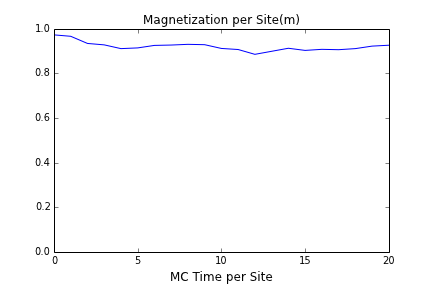
\includegraphics[width=\textwidth]
                {../../programs/graphics/equilibration_time/magnet_allup_T2,000000.png}
                \caption{Magnetization per Site vs MC Time per Site when T = 
                2.0 with all up initial spins corresponds to T=0}
        \end{subfigure}%
        ~ %add desired spacing between images, e. g. ~, \quad, \qquad etc.
          %(or a blank line to force the subfigure onto a new line)
        \begin{subfigure}[b]{0.5\textwidth}
                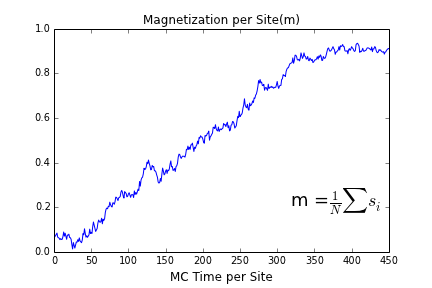
\includegraphics[width=\textwidth]
                {../../programs/graphics/equilibration_time/magnet_random_T2,000000.png}
                \caption{Magnetization per Site vs MC Time per Site when T = 
                2.0 withn random initial spins corresponds to T=$\infty$}
        \end{subfigure}
\end{figure}

\end{frame}\note{

In figure (a), we arrange initial spins to be all up, corresponds to T=0, and 
we can see that after about 5 MC Time per site, we achieve equilibrium. 
Also, in figure (b), we arrange initials spins to be random, corresponds to 
T=$\infty$, and we can see that after abot 350 MC Time per site, we 
achieve equilibrium, when our system's temperature is 2.0. Hence, if we 
initial temperature of the system's is close to the our system's temperature, 
we get equilibrium faster. 

(T = 2.0 ( Tˆ = kT) ( we wrote T=2.0 instead of Tˆ=2.0 ))

//// cıkarılabilir burası da
We want to analyze Ising Model for a lot of temperatures; hence, starting 
simulation with spin configuration at the end of the simulation for previous 
temperature, will decrease our equilibration time
}

\subsection{Autocorrelation Function and Correlation Time}
\begin{frame}
\frametitle{Autocorrelation Function and Correlation Time}
Autocorrelation function for magnetization is,
\begin{figure}
        \centering
        \begin{subfigure}[b]{0.5\textwidth}
                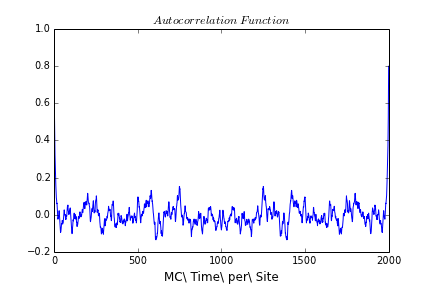
\includegraphics[width=\textwidth]
                {../../programs/graphics/autocorrelation/autocorrelation_T2,000000.png}
                \caption{Autocorrelation function vs MC Time per Site when T = 
                2.0}
        \end{subfigure}%
        ~ %add desired spacing between images, e. g. ~, \quad, \qquad etc.
          %(or a blank line to force the subfigure onto a new line)
        \begin{subfigure}[b]{0.5\textwidth}
                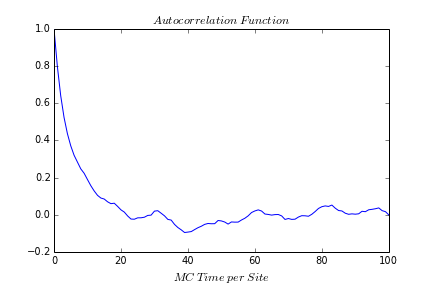
\includegraphics[width=\textwidth]
                {../../programs/graphics/autocorrelation/autocorrelation2_T2,000000.png}
                \caption{Autocorrelation function vs MC Time per Site when T = 
                2.0}
        \end{subfigure}
\end{figure}


\end{frame}
\note{

To determine correlation time, we should consider autocorrelation 
function. We expect that normalized autocorrelation function is in the form 
of e^-(t/tau) at early time steps. Hence, in the figures we can see this 
proportionality. 

Autocorrelation niye simetrik oldugu acıklanmalı. 


}

\begin{frame}
Fitting autocorrelation function for early times,
\begin{figure}
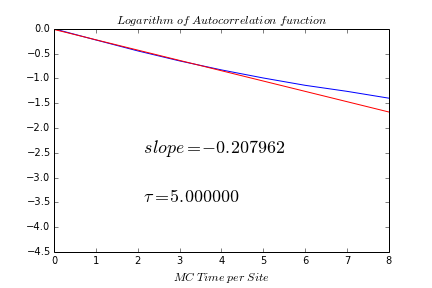
\includegraphics[scale=0.6] 
{../../programs/graphics/autocorrelation/correlation_fit_T2,000000.png}
\caption{$log(\frac{\chi (t)}{\chi (0)})$ vs MC Time per Site when T = 2.0}

\end{figure}
\end{frame}\note{

If we take logarithm of normalized autocorrelation function we expect that 
it is linear in time. Hence, by fitting it we can find correlation time. 

Then, by taking a sample in each τ time per site, we have independent data 
for properties of the system after reaching the equilibrium.

Using these independent samples, we can analyze them.

}

\subsection{Analysis of System Properties}
\begin{frame}
\frametitle{System's Properties}
\begin{figure}
        \centering
        \begin{subfigure}[b]{0.5\textwidth}
                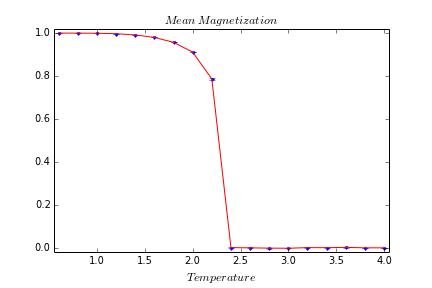
\includegraphics[width=\textwidth]
                {../../programs/graphics/properties/magnetization_L50.png}
                \caption{Mean magnetization per site vs Temperature}
        \end{subfigure}%
        ~ %add desired spacing between images, e. g. ~, \quad, \qquad etc.
          %(or a blank line to force the subfigure onto a new line)
        \begin{subfigure}[b]{0.5\textwidth}
                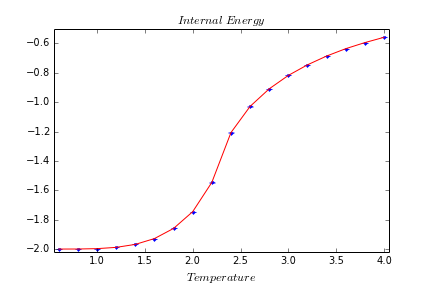
\includegraphics[width=\textwidth]
                 {../../programs/graphics/properties/internal_energy_L50.png}
                \caption{Internal energy per site vs Temperature}
        \end{subfigure}
\end{figure}
\end{frame}\note{


If we look at the plot, mean magnetization is 1 when T=0 and 0 when T=∞ 
as we expected. Also, if we increase the temperature from 0, we see that 
magnetization is about 1 until T is around 2.2. Also, if we keep on 
increasing the temperature, we will see a sharp decrease in magnetization 
to 0. This sharp change around when T is around 2.2 is called Phase 
Transition. We will discuss phase transition in the following slides.

Again, we see that a change in internal energy of the system when T is 
around 2.2. This is also caused by phase transition.


}

\begin{frame}
\begin{figure}
        \begin{subfigure}[b]{0.5\textwidth}
                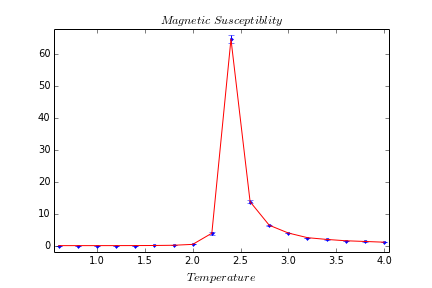
\includegraphics[width=\textwidth]
                {../../programs/graphics/properties/magnetic_suscept_L50.png}
                \caption{Magnetic suscept. vs Temperature}
        \end{subfigure}%
        ~ %add desired spacing between images, e. g. ~, \quad, \qquad etc.
          %(or a blank line to force the subfigure onto a new line)
        \begin{subfigure}[b]{0.5\textwidth}
                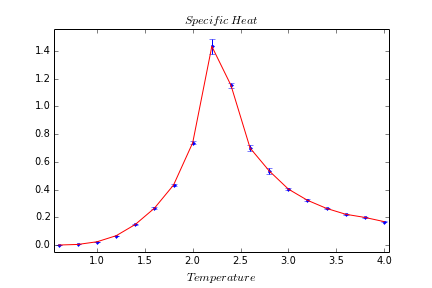
\includegraphics[width=\textwidth]
                 {../../programs/graphics/properties/specific_heat_L50.png}
                \caption{Specific heat vs Temperature}
        \end{subfigure}
\end{figure}
\end{frame}\note{

Let’s look at fluctuations in magnetization and energy, which are magnetic 
susceptibility and specific heat of the system.

Magnetic suscept:
We can see that fluctuations in the magnetization is increased at the 
temperature of phase transition. Hence, we see a peak at that temperature. 
Also, because of this increased fluctuations at the phase transition and 
increased correlation times at phase transition our error bars are increased

Specific heat:
As in magnetic susceptibilitiy, fluctuations (hence, specific heat) in energy 
is increased at the phase transition.

}

\begin{frame}
Look at correlation times:
\begin{figure}
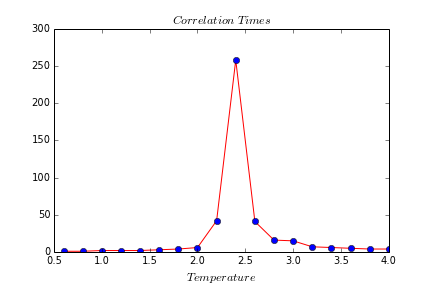
\includegraphics[scale=0.6]                  
{../../programs/graphics/properties/correlation_time_L50.png}
                \caption{Correlation time vs Temperature}

\end{figure}
\end{frame}\note{

When phase transition occurs, our correlation times, states times between 
independent states, are increased. Hence, because of that it is hard to 
simulate system around phase transition. Because, to get a lot of 
independent samples, we have to wait for a long time between independent 
samples. These increased correlation time causes us to get a small number 
of samples; hence,causes increased error bars of properties at the phase 
transition.

}

\section{Investigation of System at Critical Temperature}
\subsection{Phase Transition}
\begin{frame}
Occurs at Critical temperature $T_c$. \\
Property of Ising Model \\
For 2D Ising model, $T_c \approx 2.269$ \\
Events that occur in the critical region are called critical phenomena.  \\
Causes critical fluctuations

\end{frame}\note{

We have seen that at phase transition, our correlation times diverge, there is a sharp change in magnetization and energy, hence there is a divergence in the magnetic susceptibility and specific heat at the phase transition. This phase transition is a property of the Ising model.

Now, suppose we are at high temperatures where spins are random and uncorrelated. If we decrease temperature, interaction between spins forces spins to be in same direction. Hence, spins become correlated. Spin groups which are correlated because of these effect are called clusters and size of clusters are ξ, correlation length. This is because of the nature of the Ising model. Hence, at the phase transition, we have a lot of spin groups, seperately. If we continue to decrease temperature, spins chose a direction and generate non-zero magnetization. When T goes to 0 , the most of the spins are in same direction and absolute magnetization per spin goes to 1.

We know that when temperature is high our spins are random when we are approach critical temperature from there, clusters occur, clusters includes spins that are correlated. Hence, when we flip a spin at critical temperature, these clusters flip, because spins inside it are correlated, hence, we see fluctuations in magnetization and energy, these fluctuations are called critical fluctuations. Thus, when we are approaching critical temperature from a high temperature, ξ increases and fluctuations increase, hence magnetic susceptibility and specific heat increases. One of the error sources in critical region is these fluctuations.

The other source of error is correlation time. At critical temperature, most of the spins are correlated to each other and with Metropolis algorithm we flip spins one by one. Hence, to get a state which is independent of current state, we have to wait a long correlation time. These long correlation time causes errors in calculation since we need a lot of independent measurements in simula- tion and when correlation times increase, we get lower measurements and because of that, error becomes higher. Actually, in thermodynamical limit correlation time diverges, but in our case, where finite size exists, correlation time becomes very high. This increase in correlation time is called Critical slowing down. This error source is depend on our algo- rithm whereas, fluctuation is a property of system. Hence, we can find a way to decrease correlation times to increase accuracy.

}

\subsection{Critical Exponents}
\begin{frame}
\frametitle{Critical Exponents}
When we approach to phase transition correlation length increases. \\
Reduced temperature, $t$, is
\begin{equation}
t = \frac{T- T_c}{T_c}
\end{equation}
For Ising model, divergence of correlation length near phase transition goes like
\begin{equation}
\xi \propto |t|^{-\nu}
\end{equation}
$\nu$ is critical exponent.
Correlation Time per site 
\begin{equation}
\tau \propto |t|^{-z \nu} \propto \xi^{z}
\end{equation}
z is dynamic exponent.
\end{frame}\note{

ν is critical exponent and is a property of Ising model, independent of J or lattice size, algorithm, ... . This is known as universality. Hence, ξ depends only on nature of Ising model.

Hence, with using dynamic exponent, we can analyze critical slowing down effect.
Also, we know that critical slowing down depends on our algorithm. Hence, z depends on our algorithm, then, we want small z values in our algorithm. If z = 0, there is no critical slowing down and we can simulate Ising model around phase transition, efficiently.
If we know critical temperature analitically, to measure critical exponents, we should look at finite size scaling.
}

\subsection{Finite Size Scaling}
\begin{frame}
\frametitle{Finite Size Scaling}
\begin{equation}
\tau \propto L^{z}
\end{equation} 
\begin{figure}
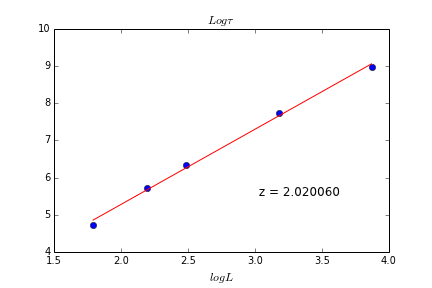
\includegraphics[scale=0.6]                  {../../programs/graphics/properties/dynamic_exponent.png}
                \caption{$Log\tau$ vs $LogL$}

\end{figure}



\end{frame}\note{
We know that ξ diverges near phase transition; hence, correlation times near phase transi- tion are getting bigger.

In Monte Carlo simulations, we simulate models within a finite size. Because of finite size, correlation times actually can never really diverge. In a simulation, maximum value of correlation length is Ld, where d is dimension of our system. Therefore, when we are at critical temperature, our correlation length is approximatelly L2 for an 2D Ising model.

At T = Tc, if we plot correlation times with respect to L on logarithmic scale, we can get z.
For Metropolis Algorithm: z is found as 2.02. This z is a high value for Monte Carlo simulations. Hence, it causes a great critical slowing down
Now, with using different algorithms we want to decrease dynamic exponent values, hence, want to decrease correlation times.

If we look at Wolff algorithm, we get a lower value of z, hence, we expect that Wolff algorithm is better than Metropolis algorithm near phase transition. When, we are away from critical temperature (Tc) Metropolis algorithm is a good choice to simulate Ising model. When we approach to Tc, correlation times are getting bigger and it makes hard to get sufficient independent values. Hence, because of this effect errors increase when we approach the phase transition.
}

\subsection{Wolff Algorithm}
\begin{frame}
\frametitle{Wolff Algorithm}
Cluster-flipping algorithm \\
Look for clusters of similarly oriented spins and then flip them in their entirely all in one go, rather than trying to turn them over spin by spin.
\end{frame}\note{

The reason of that z is high values in Metropolis algorithm is because of divergence of correlation length ξ and critical fluctations near phase transition. When T is closer to critical temperature, correlation length is getting bigger and large regions of spins are in same direction. This regions are called domains. When T = Tc , J = 0.44 ; hence, Tc = 2, 269J, A(μ → ν) ≈ e−8J/Tc ≈ 0.03 This is about 3 percent to flip a spin inside a domain. Therefore, for Metropolis algorithm it is difficult to flip a spin because it tries to flip spin by spin. As a result of this, acceptance ratio is very low around critical temperature and generally, we don’t change state. Because of this, simulation time diverges around critical temperature.

Also, chance of flip a spin at the edge of a domain is high because it has opposite spins in its neighbourhood, hence lower energy cost. The basic idea of Wolff algorithm is to look for clusters of similarly oriented spins and then flip them in their entirely all in one go, rather than trying to turn them over spin by spin.

With using Cluster algorithms we can get rid of critical slowing down.


oku ve yaz wolff u 
}

\begin{frame}
Wolff Algorithm,
\begin{enumerate}
\item Select a spin randomly.
\item Look at the neighboring spins. If they are in same direction, add the cluster with probability $P_{add}$
\item For a spin that is added to the cluster, look at the neighboring spins of this spin and again add the spins with same direction which are not in the cluster with probability $P_{add}$
\item Repeat the process and complete the cluster
\item Flip the cluster
\end{enumerate}
To make a fair description of $\tau$
\begin{equation}
\tau = \tau_{steps} \frac{\langle n \rangle }{L^d}
\end{equation}
\end{frame}\note{
After, defining initial spins we can start the simulation.

Now, we expect that correlation times to decrease when Wolff algorithm is used. To
see, it we can compare dynamic exponents of Wolff algorithm and Metropolis algorithm.


In Wolff algorithm we flip spins in a cluster. If there is n spins in a cluster, we flip n spins. Also, in Metropolis algorithm we flip 1 spin. Hence, to make a fair description of correlation time, this difference must be considered. We calculated correlation times for Metropolis algorithm in MC time per site. Thus, to achieve an independent state, we have to wait τ trials of flipping 1 spin, per spin, in scrictly speaking. Also, again if we calculate correlation times for Wolff algorithm as in Metropolis algorithm, again we have to wait tau/(<n>/L^d)  trials of flipping 1 spin, per spin. Hence, if we multiply which is found in Wolff algorithm with <n>/L^d we make a fair calculation of correlation time. 

Where τ_steps is found in Wolff algorithm and ⟨n⟩ is mean value of cluster sizes.

}

\begin{frame}
\begin{equation}
\tau \propto L^{z}
\end{equation} 
\begin{figure}
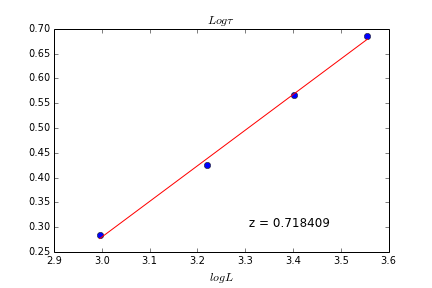
\includegraphics[scale=0.6]                  {../../programs/graphics/properties/dynamic_exponent_wolff.png}
                \caption{$Log\tau$ vs $LogL$}

\end{figure}
\end{frame}\note{

Now, we can compare Wolff and Metropolis algorithms in the critical region. If we look at dynamic exponent values for two algorithms, then we can see that, for Metropolis algorithm z = 2.02 and for Wolff algorithm z = 0.72. We know that τ ∝ Lz at critical temperature for a finite size system. Hence, we can see that at critical temperature Wolff algorithm’s correlation time is much lower than Metropolis algorithm’s. Also, CPU time to simulate one correlation time for 2D Ising model is τCPU ∝ L2+z, hence, CPU time is, also, much lower for Wolff algorithm. Besides, we can compare correlation times that we found for two algorithms. For instance, for a 20x20 lattice, with Metropolis algorithm τ = 1040 MC step per site and with Wolff algorithm τ = 4 MC step per site, at critical temperature. There is a huge difference in correlation time values for two algorithms.
If we want to analyze behaviour of the model at Tc, a cluster spin algorithm, such as Wolff algorithm, is more efficient than a single spin algorithm, such as Metropolis algorithm.

}


\end{document}











